\UseRawInputEncoding
\documentclass[a4paper, 14pt]{extarticle}

% Поля
%--------------------------------------
\usepackage{geometry}
\geometry{a4paper,tmargin=2cm,bmargin=2cm,lmargin=3cm,rmargin=1cm}
%--------------------------------------


%Russian-specific packages
%--------------------------------------
\usepackage[T2A]{fontenc}
\usepackage[utf8]{inputenc} 
\usepackage[english, main=russian]{babel}
%--------------------------------------

\usepackage{textcomp}

% Красная строка
%--------------------------------------
\usepackage{indentfirst}               
%--------------------------------------             


%Graphics
%--------------------------------------
\usepackage{graphicx}
\graphicspath{ {./images/} }
\usepackage{wrapfig}
%--------------------------------------

% Полуторный интервал
%--------------------------------------
\linespread{1.3}                    
%--------------------------------------

%Выравнивание и переносы
%--------------------------------------
% Избавляемся от переполнений
\sloppy
% Запрещаем разрыв страницы после первой строки абзаца
\clubpenalty=10000
% Запрещаем разрыв страницы после последней строки абзаца
\widowpenalty=10000
%--------------------------------------

%Списки
\usepackage{enumitem}

%Подписи
\usepackage{caption} 

%Гиперссылки
\usepackage{hyperref}

\hypersetup {
	unicode=true
}

%Рисунки
%--------------------------------------
\DeclareCaptionLabelSeparator*{emdash}{~--- }
\captionsetup[figure]{labelsep=emdash,font=onehalfspacing,position=bottom}
%--------------------------------------

\usepackage{tempora}
\usepackage{amsmath}
\usepackage{color}
\usepackage{listings}
\lstset{
  belowcaptionskip=1\baselineskip,
  breaklines=true,
  frame=L,
  xleftmargin=\parindent,
  language=Python,
  showstringspaces=false,
  basicstyle=\footnotesize\ttfamily,
  keywordstyle=\bfseries\color{blue},
  commentstyle=\itshape\color{purple},
  identifierstyle=\color{black},
  stringstyle=\color{red},
  extendedchars=\true,
}

%--------------------------------------
%			НАЧАЛО ДОКУМЕНТА
%--------------------------------------

\begin{document}

%--------------------------------------
%			ТИТУЛЬНЫЙ ЛИСТ
%--------------------------------------
\begin{titlepage}
\thispagestyle{empty}
\newpage


%Шапка титульного листа
%--------------------------------------
\vspace*{-60pt}
\hspace{-65pt}
\begin{minipage}{0.3\textwidth}
\hspace*{-20pt}\centering

\includegraphics[width=\textwidth]{emblem}
\end{minipage}
\begin{minipage}{0.67\textwidth}\small \textbf{
\vspace*{-0.7ex}
\hspace*{-6pt}\centerline{Министерство науки и высшего образования Российской Федерации}
\vspace*{-0.7ex}
\centerline{Федеральное государственное бюджетное образовательное учреждение }
\vspace*{-0.7ex}
\centerline{высшего образования}
\vspace*{-0.7ex}
\centerline{<<Московский государственный технический университет}
\vspace*{-0.7ex}
\centerline{имени Н.Э. Баумана}
\vspace*{-0.7ex}
\centerline{(национальный исследовательский университет)>>}
\vspace*{-0.7ex}
\centerline{(МГТУ им. Н.Э. Баумана)}}
\end{minipage}
%--------------------------------------

%Полосы
%--------------------------------------
\vspace{-25pt}
\hspace{-35pt}\rule{\textwidth}{2.3pt}

\vspace*{-20.3pt}
\hspace{-35pt}\rule{\textwidth}{0.4pt}
%--------------------------------------

\vspace{1.5ex}
\hspace{-35pt} \noindent \small ФАКУЛЬТЕТ\hspace{80pt} <<Информатика и системы управления>>

\vspace*{-16pt}
\hspace{47pt}\rule{0.83\textwidth}{0.4pt}

\vspace{0.5ex}
\hspace{-35pt} \noindent \small КАФЕДРА\hspace{50pt} <<Теоретическая информатика и компьютерные технологии>>

\vspace*{-16pt}
\hspace{30pt}\rule{0.866\textwidth}{0.4pt}
  
\vspace{11em}

\begin{center}
\Large {\bf Лабораторная работа КР-1} \\ 
\large {\bf<<Мобильно приложение, реализующее метод Карацубы>>} \\ 
\large {\bf по курсу <<Численные методы линейной алгебры>>} \\ 
\end{center}\normalsize

\vspace{8em}


\begin{flushright}
  {Студент группы ИУ9-71Б Лысенко В. В.\hspace*{15pt} \\
  \vspace{2ex}
  Преподаватель Посевин Д. П.\hspace*{15pt}}
\end{flushright}

\bigskip

\vfill
 

\begin{center}
\textsl{Москва 2024}
\end{center}
\end{titlepage}
%--------------------------------------
%		КОНЕЦ ТИТУЛЬНОГО ЛИСТА
%--------------------------------------

\renewcommand{\ttdefault}{pcr}

\setlength{\tabcolsep}{3pt}
\newpage
\setcounter{page}{2}

\section{Цель работы}\label{Sect::task}
\par
\renewcommand{\labelenumii}{\arabic{enumi}.\arabic{enumii}.}
Разработать мобильное приложение на Kotlin или Dart, реализующее метод А.А. Карацубы для перемножения длинных чисел.


\section{Практическая реализация}
Dart-приложение содержит 2 поля ввода для целых чисел; 2 текстовые строки, содержащие двоичное представление введённых чисел; 2 текстовых поля, содержащие информацию о времени отработки алгоритма Карацубы и обычного перемножения чисел; а также текстовое поле, демонстрирующее результат умножения.

\par
Код программы:
\begin{lstlisting}
import 'dart:math';
import 'package:flutter/material.dart';

void main() {
  runApp(KaratsubaApp());
}

class KaratsubaApp extends StatelessWidget {
  @override
  Widget build(BuildContext context) {
    return MaterialApp(
      debugShowCheckedModeBanner: false,
      title: 'Karatsuba',
      home: KaratsubaScreen(),
    );
  }
}

class KaratsubaScreen extends StatefulWidget {
  @override
  _KaratsubaScreenState createState() => _KaratsubaScreenState();
}

class _KaratsubaScreenState extends State<KaratsubaScreen> {
  final _uController = TextEditingController();
  final _vController = TextEditingController();

  String _binaryU = '';
  String _binaryV = '';
  String _normal_time = '';
  String _karatsuba_time = '';
  String _result = '';

  String _toBinary(BigInt number) => number.toRadixString(2);

  BigInt _longMultiplication(BigInt u, BigInt v) {
    List<int> uDigits = u.toString().split('').map(int.parse).toList();
    List<int> vDigits = v.toString().split('').map(int.parse).toList();

    List<int> result = List.filled(uDigits.length + vDigits.length, 0);

    for (int i = uDigits.length - 1; i >= 0; i--) {
      for (int j = vDigits.length - 1; j >= 0; j--) {
        int product = uDigits[i] * vDigits[j];
        int posLow = i + j + 1;
        int posHigh = i + j;

        product += result[posLow];
        result[posLow] = product % 10;
        result[posHigh] += product ~/ 10;
      }
    }

    BigInt finalResult = BigInt.zero;
    for (int digit in result) {
      finalResult = finalResult * BigInt.from(10) + BigInt.from(digit);
    }

    return finalResult;
  }

  BigInt _karatsuba(BigInt u, BigInt v) {
    if (u.bitLength <= 64 || v.bitLength <= 64) {
      return u * v;
    }

    int n = max(u.bitLength, v.bitLength);
    int m = (n ~/ 2);

    BigInt high1 = u >> m;
    BigInt low1 = u - (high1 << m);
    BigInt high2 = v >> m;
    BigInt low2 = v - (high2 << m);

    BigInt z0 = _karatsuba(low1, low2);
    BigInt z1 = _karatsuba((low1 + high1), (low2 + high2));
    BigInt z2 = _karatsuba(high1, high2);

    return (z2 << (2 * m)) + ((z1 - z2 - z0) << m) + z0;
  }

  void _calculate() {
    setState(() {
      BigInt? u = BigInt.tryParse(_uController.text);
      BigInt? v = BigInt.tryParse(_vController.text);

      if (u == null || v == null) {
        _binaryU = '';
        _binaryV = '';
        _normal_time = 'Invalid input';
        _karatsuba_time = 'Invalid input';
        _result = 'Invalid input';
        return;
      }

      _binaryU = _toBinary(u);
      _binaryV = _toBinary(v);

      final naiveStopwatch = Stopwatch()..start();
      BigInt naiveResult = _longMultiplication(u, v);
      naiveStopwatch.stop();
      _normal_time = '${naiveStopwatch.elapsedMicroseconds} мс';

      final karatsubaStopwatch = Stopwatch()..start();
      BigInt karatsubaResult = _karatsuba(u, v);
      karatsubaStopwatch.stop();
      _karatsuba_time = '${karatsubaStopwatch.elapsedMicroseconds} мс';

      _result = karatsubaResult.toString();
    });
  }

  @override
  Widget build(BuildContext context) {
    return Scaffold(
      appBar: AppBar(title: Text('Метод А.А. Карацубы')),
      body: Center(
        child: Padding(
          padding: const EdgeInsets.all(16.0),
          child: SingleChildScrollView(
            child: Column(
              mainAxisAlignment: MainAxisAlignment.center,
              children: [
                TextField(
                  controller: _uController,
                  decoration: InputDecoration(labelText: 'U: '),
                  keyboardType: TextInputType.number,
                ),
                TextField(
                  controller: _vController,
                  decoration: InputDecoration(labelText: 'V:'),
                  keyboardType: TextInputType.number,
                ),
                SizedBox(height: 20),
                Text('Двоичное представление u: $_binaryU'),
                SizedBox(height: 10),
                Text('Двоичное представление v: $_binaryV'),
                SizedBox(height: 20),
                Text('Время отработки (метода Карацубы): $_karatsuba_time'),
                SizedBox(height: 10),
                Text('Время отработки (обычное умножение): $_normal_time'),
                SizedBox(height: 25),
                Text('Результат умножения: $_result'),
                SizedBox(height: 10),
                ElevatedButton(
                  onPressed: _calculate,
                  child: Text('Преобразовать и умножить'),
                ),
              ],
            ),
          ),
        ),
      ),
    );
  }
}
\end{lstlisting}

\section{Результаты}
\par
Результат выполнения программы:
\begin{center}
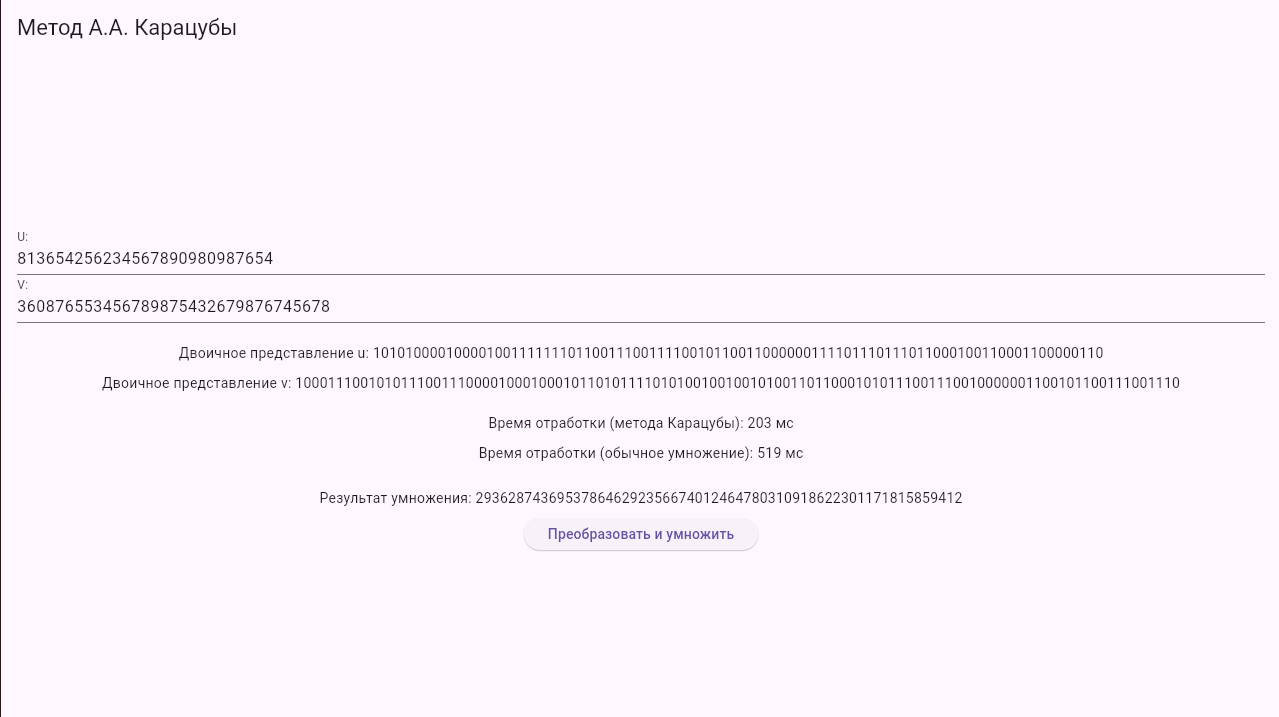
\includegraphics[scale=0.3]{g1}
\end{center}
\par


\section{Выводы}
В ходе выполнения лаборатороной работы было реализовано dart-приложение, демонстрирующее работу алгоритма А.А. Карацубы и его сравнение с обычным перемножением.
\end{document}
